\documentclass{article}
%\documentclass[journal]{IEEEtran}
%\documentclass{report}
%\documentclass{acta}
\usepackage[linktoc=all]{hyperref}
\usepackage{graphicx}
\usepackage[utf8]{inputenc}
\usepackage{subfigure}
\usepackage{alltt}
\usepackage{color}
\usepackage{url}
\newcommand{\todo}[1]{\textbf{\textsc{\textcolor{red}{(TODO: #1)}}}}

\begin{document}

\title{Aufgabe 1 \\ Machine Learning for Visual Computing}
\author{Philipp Omenitsch, Thomas Pinetz and Andreas Mair}

\pagenumbering{roman}


\maketitle
\begin{abstract}
Abgabe 1 für Machine Learning for Visual Computing über die Themen Datengenerierung, einfacher Klassifikator und Perzeptron.
\end{abstract}

\tableofcontents
\clearpage
\pagenumbering{arabic}

\section{Datengenerierung}
\label{ch:atengenerierung}

Die Generierung der Daten erfolgt unter Verwendung zweier Normalverteilungen. Dabei werden der Funktion die Mittelwerte sowie die Kovarianzen der Normalverteilungen �bergeben.
Anschlie�end erfolgt eine Zuteilung der Datenpunkte in zwei Klassen. Dazu wird der Richtungsvektor vom ersten Mittelwert zum zweiten Mittelwert berechnet. Dann werden die Datenpunkte, deren Mittelpunkt auf den Koordinatenursprung verschoben wurde, auf den normierten Richtungsvektor projiziert.
Alle Punkte die nun vor dem Nullpunkt liegen werden der ersten Klasse, jene die nach dem Nullpunkt liegen der zweiten Klasse zugeteilt. Falls die Klassen dadurch unterschiedlich gro� werden, wird die Entscheidungsgrenze (in sich vermindernden Schritten) vom Nullpunkt wegbewegt, bis die Klassen gleich gro� werden.
Falls die Mittelwerte gleich w�ren und somit kein Richtungsvektor berechnet werden kann, wird statt diesem der erste Eigenvektor einer PCA verwendet.
Nat�rlich erfolgt diese Aufteilung der Daten nur wenn diese linear separierbar sein sollen, falls nicht werden alle Punkte der ersten Normalverteilung der ersten Klasse und jende der zweiten Normalverteilung der zweiten Klasse zugeteilt.

\subsection{Darstellung der Datenvektoren und ihrer Labels als Plot}

\begin{figure}
	
	\centering
	\mbox{
		\subfigure[Leicht separierbare Daten]{
			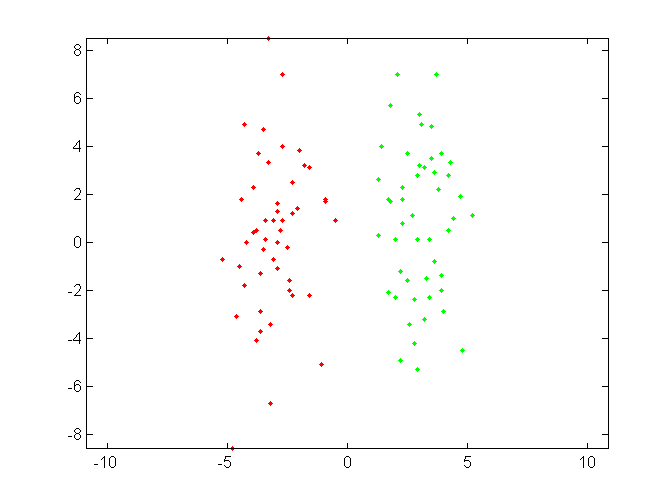
\includegraphics[width=60mm, trim = 0cm 0cm 0cm 0cm]{img/task1simple.png}
		}
		
		\subfigure[Separierbar trotz gleicher Mittelwerte und Kovarianzen]{
			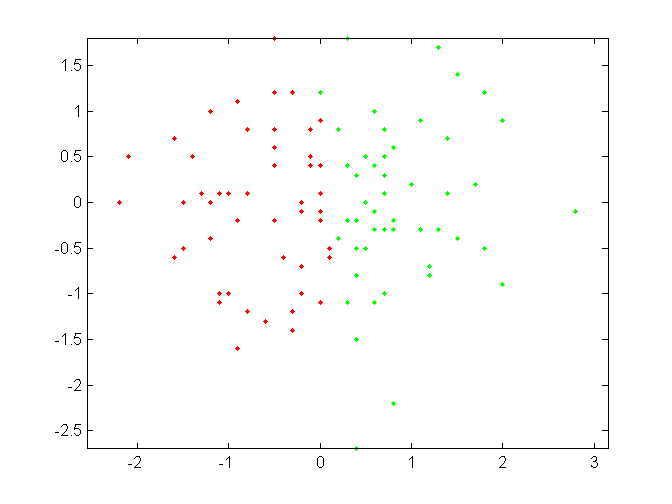
\includegraphics[width=60mm, trim = 0cm 0cm 0cm 0cm]{img/task1close.png}
		}	
	}
	\mbox{
		\subfigure[Nicht linear separierbar]{
			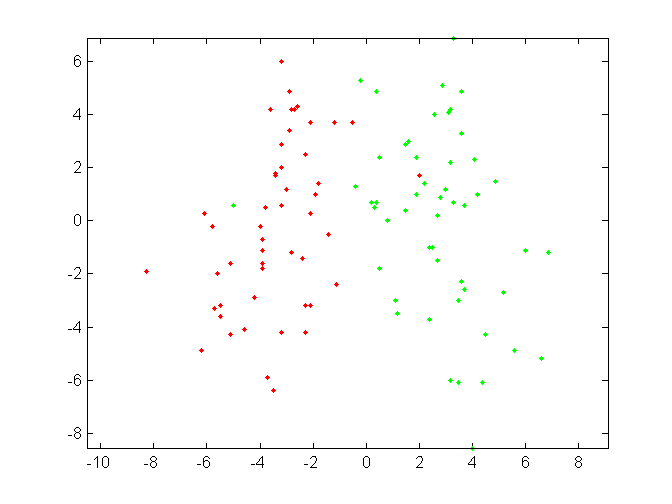
\includegraphics[width=60mm, trim = 0cm 0cm 0cm 0cm]{img/task1notsep.png}
		}
	}
	
	\caption{Darstellung der Datenvektoren und ihrer Labels als Plot}
	\label{fig:gendata}
\end{figure}
\section{Einfacher Klassifikator}
\label{ch:implementation}

Der einfache Klassifikator stellt in unserem Fall eine memory Funktion da. Das heißt, dass wenn wir einen Datensatz schon gesehen haben, geben wir dessen Werte aus. Wenn wir diesen noch nicht gesehen haben geben wir einen negativen Wert zurück. Nachdem wir alle möglichen Zahlenkombinationen gesehen haben, haben wir einen perfekten Klassifikator. 



\subsection{Warum overfitted die Funktion memory? Was bedeutet Overfitting in Zusammenhang mit dem Lernen von Klassifikatoren?} 

Der Klassifikator hat auf dem Trainingset 100 \% da er die selben Werte wiedererkennt. Dafür kann man mit diesem Klassifikator nicht generalisieren. Wenn auch nur einer der Werte minimal abweicht bekommt man immer einen negativen Returnwert obwohl es eigentlich viel wahrscheinlicher ist, dass dieser Wert den selben output wert hat als sein minimal unterschiedlicher Nachbar. Daher kann man mit diesem Klassifikator nicht generalisieren.Durch die fehlende Generalisierung werden viele Daten falsch klassifieziert. Dadurch ist die Performance außerhalb des Testsets, wie man bei unseren Resultaten sehen kann sehr schlecht. 


\chapter{Ergebnisse}
\label{ch:results}

In diesem Abschnitt werden nun die von uns gefundenen Ergebnisse dargestellt und diskutiert.

\section{Verwendung aller Features}

Zuerst betrachten wir die Ergebnisse der einzelnen Klassifikatoren, um optimale Parameter zu finden.

\subsection{k-Nearest-Neighbor}

Beim k-Nearest-Neighbor-Klassifikator haben wir empirisch untersucht, wie sich eine Veränderung des $k$-Wertes im Ergebnis und der Laufzeit niederschlägt. Das Ergebnis ist in nachstehender Tabelle dargestellt:

\begin{center}
	\begin{tabular}{ | c | c | c | c | c | }
		\hline
		\textbf{k} & \textbf{Laufzeit} & \textbf{False Positives} & \textbf{False Negatives} & Richtige Zuordnung \\ \hline
		1 & 7,771272 & 3,9046 \% & 3,6876 \% & 92,4078 \% \\ \hline
		2 & 7,683023 & 1,7354 \% & 6,7245 \% & 91,5401 \% \\ \hline
		3 & 7,675488 & 3,6876 \% & 4,7722 \% & 91,5401 \% \\ \hline
		4 & 7,689970 & 1,7354 \% & 6,5076 \% & 91,7570 \% \\ \hline
		5 & 7,711205 & 2,8200 \% & 4,9892 \% & 92,1909 \% \\ \hline
	\end{tabular}
\end{center}

Wie man sieht, hat die Wahl des Wertes von $k$ keinen Einfluss auf die Laufzeit. Dies ist auch intuitiv einleuchend, da die Ergebnisse ohnehin nach Entfernung sortiert werden müssen und es daher von der Laufzeitkomplexität keinen wesentlichen Unterschied macht, ob nun jene $n$ Ergebnisse herangezogen werden, die am nähesten liegen, oder eben $n+1$ Ergebnisse. Sehr wohl hingegen kann man einen Unterschied bei den Klassifikationsergebnissen ausmachen. Da das Ergebnis für den \textit{False Positive}-Wert bei einem $k$-Wert von 2 am geringsten ist, verwenden wir diesen für den Klassifikator.

\subsection{Perceptron}

Beim Perceptron-Klassifikator haben wir untersucht, wie sich die Anzahl der Epochen sowohl auf die Laufzeit als auch das Klassifikationsergebnis auswirkt. Wie sich zeigt ist die Laufzeit, die für das Trainieren des Klassifikators notwendig ist, annähernd linear. Das interessanteste Ergebnis ist jedoch, dass das Verhältnis der False-Positive-Klassifikationen zu der Gesamtanzahl der Daten im Test-Set anfangs sehr stark abnimmt, mit zunehmender Anzahl an Epochen jedoch immer nur noch schwächere Verbesserungen bringt. Auch hinsichtlich des Gesamtergebnisses bringt eine zunehmende Steigerung der Epochen-Anzahl über einen bestimmten Wert hinaus keine signifikanten Veränderungen mehr. Die Ergebnisse sind zusammenfassend in Bild~\ref{fig:perceptron} dargestellt.

\begin{figure}
	
	\centering
	\mbox{
		\subfigure[Auswirkung auf die False Positives und False Negatives]{
			\includegraphics[width=60mm, trim = 0cm 0cm 0cm 0cm]{../Practical/plots/perc_epochen_false.png}
		}
		
		\subfigure[Auswirkung auf das Gesamtergebnis]{
			\includegraphics[width=60mm, trim = 0cm 0cm 0cm 0cm]{../Practical/plots/perc_epochen_right.png}
		}	
	}
	\mbox{
		\subfigure[Auswirkung auf die Laufzeit]{
			\includegraphics[width=60mm, trim = 0cm 0cm 0cm 0cm]{../Practical/plots/perc_epochen_runtime.png}
		}
	}
	
	\caption{Performence des Perceptron-Klassifizierers in Abhängigkeit der Epochen.}
	\label{fig:perceptron}
\end{figure}

\subsection{Mahalanobis-Distanz}

Da es bei dem Klassifikationsverfahren mit der Mahalanobis-Distanz keine weiteren Parameter gibt, die man modifzieren kann, ist hier nur das Gesamtergebnis des Klassifkatiors dargestellt:

\begin{center}
	\begin{tabular}{ | c | c | c | }
		\hline
		False Positives & False Negatives & Richtige Zuordnung \\
		\hline
		6,07 \% & 6,51 \% & 87,42 \% \\		
		\hline
	\end{tabular}
\end{center}


\section{Egebnisse nach Feature-Reduzierung}

In diesem Abschnitt werden die Ergebnisse unserer beiden in Abschnitt \ref{sec:feature_red} erwähnten Verfahren besprochen, mit der die Anzahl der Features reduziert werden soll.

\subsection{Entfernung von Features mit geringer Varianz}

Mit dieser Methode konnten wir recht gute Ergebnisse erzielen. Abhängig von dem gewählen Klassifikationsverfahren lassen sich auch noch akzeptable Ergebnisse mit einer deutlich reduzierten Anzahl an Features erreichen. Die folgende Tabelle gibt eine Übersicht, wie viele Features bei welcher Grenze noch übrig geblieben sind:

\begin{center}
	\begin{tabular}{ | c | c |  }
		\hline
		\textbf{Grenze für Varianz} & \textbf{Anzahl Features} \\ \hline
		0 & 58 \\ \hline
		0.1 & 44 \\ \hline
		0.2 & 31 \\ \hline
		0.3 & 23 \\ \hline
		0.4 & 19 \\ \hline
		0.5 & 16 \\ \hline
		1 & 10 \\ \hline
		2 & 7 \\ \hline
	\end{tabular}
\end{center}

Die Werte für die \textit{False Positive}, \textit{False Negative} sowie die Gesamtanzahl der korrekt kategorisierten Ergebnisse sind in Bild~\ref{fig:featurereduce} dargestellt.

\begin{figure}
	
	\centering
	\mbox{
		\subfigure[kNN]{
			\includegraphics[width=60mm, trim = 0cm 0cm 0cm 0cm]{../Practical/plots/feat_reduce_knn.png}
		}
		
		\subfigure[Perceptron]{
			\includegraphics[width=60mm, trim = 0cm 0cm 0cm 0cm]{../Practical/plots/feat_reduce_perceptron.png}
		}	
	}
	\mbox{
		\subfigure[Mahalanobis]{
			\includegraphics[width=60mm, trim = 0cm 0cm 0cm 0cm]{../Practical/plots/feat_reduce_maha.png}
		}
		
		\subfigure[Zusammengefasst]{
			\includegraphics[width=60mm, trim = 0cm 0cm 0cm 0cm]{../Practical/plots/feat_reduce_right.png}
		}	
	}
	
	\caption{Darstellung der Ergebnisse der Feature-Reduktion für die einzelnen Klassifikatoren.}
	\label{fig:featurereduce}
\end{figure}

\subsection{Schrittweise Entfernung des Features mit dem geringsten Effekt}

Diese Methode ist sehr rechenintensiv, da man, um jenes Feature auswählen zu können, welches Entfernt werden soll, das Gesamtergebnis bei $n$ Features $n$ mal berechnen muss. Wir haben uns daher entschlossen, zuerst nur für den Perceptron-Classifier anzuwenden, um abschätzen zu können, wie erfolgsversprechend dieses Verfahren ist.

\begin{center}
	\begin{tabular}{ | c | c | c | c | }
		\hline
		Entfernte(s) Feature(s) & False Positives & False Negatives & Richtige Zuordnung \\ \hline
		17 & 4,1215 \% & 5,4230 \% & 90,4555 \% \\ \hline
		17,44 & 4,3384 \% & 5,4230 \% & 90,2386 \% \\ \hline
		17,44,42 & 4,9892 \% & 5,2061 \% & 89,8048 \% \\ \hline
		17,44,42,1 & 4,9892 \% & 5,4230 \% & 89,5879 \% \\ \hline
		17,44,42,1,2 & 4,9892 \% & 4,9892 \% & 90,0217 \% \\ \hline
	\end{tabular}
\end{center}

Wie aus der Tabelle ersichtlich ist, kann diese Methode keinen der Werte entscheidend verbessern. Angesichts der Nachteile (Lange Laufzeit und keine signifikante Veränderung der Ergebnisse) haben wir uns entschlossen, diese Methode nicht weiter zu verfolgen.

\subsection{Auswirkung der Feature-Größe auf die Laufzeit}
\label{subsect:feat_runtime_fx}
Unabhängig von der konkreten Auswahl der Features haben wir auch untersucht, wie sich eine Reduzierung der Features auf die Laufzeit auswirkt. Die Ergebnisse sind in Bild \ref{fig:runtime} dargestellt. Das wichtigste Ergebnis ist hierbei, dass sich die Laufzeit für alle drei Klassifikationsverfahren in dem von uns untersuchten Bereich annähernd linear entwickelt.

\begin{figure}
	
	\centering
	\mbox{
		\subfigure[kNN]{
			\includegraphics[width=60mm, trim = 0cm 0cm 0cm 0cm]{../Practical/plots/runtime_knn.png}
		}
		
		\subfigure[Perceptron]{
			\includegraphics[width=60mm, trim = 0cm 0cm 0cm 0cm]{../Practical/plots/runtime_perceptron.png}
		}	
	}
	\mbox{
		\subfigure[Mahalanobis]{
			\includegraphics[width=60mm, trim = 0cm 0cm 0cm 0cm]{../Practical/plots/runtime_mahalanobis.png}
		}
		
		\subfigure[Zusammengefasst]{
			\includegraphics[width=60mm, trim = 0cm 0cm 0cm 0cm]{../Practical/plots/runtime_combined.png}
		}	
	}
	
	\caption{Darstellung der Laufzeiten der einzelnen Klassifikationsverfahren im Zusammenhang mit der Anzahl der Features.}
	\label{fig:runtime}
\end{figure}

\bibliographystyle{alpha}
\bibliography{scientific_report}


\end{document}



